%!TEX program = xelatex
%!LW recipe=latexmk (xelatex)
% LTeX: enabled=true

\documentclass[10pt]{article}

\input{style.sty}

\title{TEQUILA Commissioning Report}
\author{Alan M. Watson \& Noémie Globus}
\date{11 March 2026}

\begin{document}

\maketitle

\section{Measured Performance}

\subsection{Read Mode and SOFTGAIN}

All of the tests here were performed with a TCS read mode of \verb|0-1-128| and a \verb|SOFTGAIN| value of 16. 

The TCS read mode is three integers separated by hyphens: the first integer is the QHY SDK read mode (0 here), the seconds is the QHY SDK gain mode (0 here), and the third is the QHY SDK offset (128 here).

The raw pixel values are divided by the \verb|SOFTGAIN| immediately after reading and before any further processing; the value of 16 converts the apparent 16-bit data values returned by the SDK into 12-bit values appropriate for the actual ADC. Thus, the data values in the FITS files are in the range $[0,4095]$.

\subsection{Gain and Read-Noise}

In the laboratory on 2025-11-13 we measured a gain of 2.48 electrons/DN and a read noise of 2.6 electrons.

\subsection{Zero-Point}

We measured the zero-point by considering our observations of the star 149180247107173789 in the Pan-STARRS DR2 at $\alpha = 24.710659$ deg and $\delta = 34.319267$ deg (J2000). This star is the brightest star near GRB 260131A and appears in multiple exposures of 60 seconds taken on the night of 2026-02-01 UTC; see Figure~\ref{figure:zeropoint-star} for an example image. The star is saturated in the Pan-STARRS DR2 catalog, but has $r = 13.279 \pm 0.038$ in the APASS DR10.

We performed aperture photometry with an aperture of radius 40 pixels (3.0 arcsec) and a sky annulus between 80 and 120 pixels (6.0 and 9.0 arcsec). The mean number of counts in the aperture was $1.09\times 10^5$ with a dispersion of about 1.7\%. The dispersion possibly arises from flat-field errors or seeing or tracking variations; we do not consider it to be worrisome in this context.

With an assumed gain of 2.48 electron/DN, the zero-point is $1.24\times 10^9$ electrons/s.

\begin{figure}
    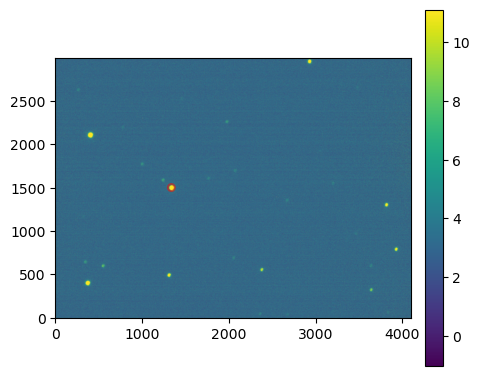
\includegraphics[width=\linewidth]{figure/zeropoint-star.png}
    \caption{The star at $\alpha = 24.710659$ deg and $\delta = 34.319267$ deg (J2000) used for the zero-point calibration is marked in red in this image.}
    \label{figure:zeropoint-star}
\end{figure}

\section{Estimated Performance}

\subsection{Photometric Performance}

In this section we construct a model for the signal-to-noise ratio for photometry. 
The signal-to-noise ratio $R_1$ in a single exposure of time $t_1$ is given by
\begin{equation}
    R_1 = \frac{Z f t_1 10^{-0.4 m}}{\sqrt{Z f t_1 10^{-0.4 m} + n_\mathrm{pix}(\sigma_\mathrm{r}^2 + r_\mathrm{sky}t_1 +  r_\mathrm{dark}t_1)}},
\end{equation}
in which $Z$ is the zero-point count rate, $f$ is the aperture correction, $n_\mathrm{pix}$ is the number of pixels in the aperture, $\sigma_\mathrm{r}$ is the read noise, $r_\mathrm{sky}$ is the count rate per pixel from the sky, and $r_\mathrm{dark}$ is the count rate per pixel from the dark current.

The zero-point count rate in $\mathrm{electron\,s^{-1}}$ was determined above to be
\begin{equation}
    Z \approx 1.24\times10^9.
\end{equation}

For a Gaussian profile, $z(r) = z(0) e^{-(r/\sigma)^2}$, we have
\begin{equation}
f = 1-e^{-(r/\sigma)^2},
\end{equation}
and the FWHM $w$ is related to $\sigma$ by $w = 2\sigma\sqrt{\ln2} \approx 1.665 \sigma$. It can be shown that the optimal aperture radius in the background-limited case is approximately $0.675 w$. That is, the optimum aperture diameter is about 1.35 times the FWHM. (Note that this aperture contains 71\% of the light, and so its diameter is quite close to $d_{80}$.)

The read noise in electrons was measured to be
\begin{equation}
    \sigma_\mathrm{r} \approx 1.8.
\end{equation}

The sky brightness $\mu$ in $r$ has been measured to be about is about $19.2\ \mathrm{mag\,arcsec^{-2}}$ in bright time and $20.7\ \mathrm{mag\,arcsec^{-2}}$ in dark time. The pixel size has been measured to be $\alpha \approx 0.076$ arcsec. Thus,
\begin{equation}
r_d = \alpha^a Z 10^{-0.4 \mu},
\end{equation}
where $\alpha$ is measured in arcsec and $\mu$ in $\mathrm{mag\,arcsec^{-2}}$. Thus, 



\end{document}
